\documentclass[10.5pt]{article}
\usepackage[letterpaper, margin=0.6in, top=0.5in, bottom=0.5in]{geometry}
\usepackage{amsmath,amssymb,amsthm}
\usepackage{fancyhdr}
\usepackage{xcolor}
\usepackage{tikz}
\usepackage{enumitem}
\usepackage{tcolorbox}
\usepackage{hyperref}

% Define colors matching instructor board annotations
\definecolor{chalkblue}{RGB}{0, 105, 185}
\definecolor{chalkred}{RGB}{205, 35, 35}
\definecolor{chalkpink}{RGB}{230, 90, 120}
\definecolor{chalkcyan}{RGB}{15, 160, 190}
\definecolor{chalkgreen}{RGB}{20, 130, 50}
\definecolor{boxbg}{RGB}{252, 252, 254}
\definecolor{boxframe}{RGB}{150, 160, 180}

\pagestyle{fancy}
\fancyhf{}
\renewcommand{\headrulewidth}{0pt}
\renewcommand{\footrulewidth}{0pt}

\setlength{\parindent}{0pt}
\setlength{\parskip}{2.5pt}

\begin{document}

% ==============================================================================
% PAGE 1 (Page 1 of 5)
% ==============================================================================
\noindent \textbf{\large Math 105L} \hfill \textbf{\large Lecture 9-2}\\[1pt]
{\textbf{\Large Implicit Differentiation}}\\[-5pt]
\rule{\textwidth}{1.2pt}

\vspace{0.03in}

\textbf{\large A Key Tool: The Chain Rule}
\vspace{-4pt}
\[
  \frac{d}{dx}\big(f(g(x))\big) = f'\big(g(x)\big) \cdot g'(x)
\]

\vspace{0.02in}

\textbf{\large Implicit Differentiation}

\begin{itemize}[leftmargin=1.2em, topsep=1pt, itemsep=1pt]
  \item \textbf{Consider the equation $xy + y = e^x$.} This defines $y$ as a function of $x$. Find $y(x)$ and use it to find $\frac{dy}{dx}$.
  \begin{itemize}[leftmargin=1.2em, label=$\bullet$, topsep=1pt, itemsep=1pt]
    \item \textbf{Solve explicitly for $y(x)$:} \quad $y(x+1) = e^x \iff y = \frac{e^x}{x+1}$
    \item \textbf{Differentiate via Quotient Rule:}
    \[
      \frac{dy}{dx} = \frac{(x+1)\frac{d}{dx}[e^x] - e^x \frac{d}{dx}[x+1]}{(x+1)^2} = \frac{(x+1)e^x - e^x(1)}{(x+1)^2} = \frac{xe^x + e^x - e^x}{(x+1)^2} = \frac{xe^x}{(x+1)^2}
    \]
  \end{itemize}
\end{itemize}

\vspace{0.03in}
\textbf{Now, consider the equation $x^2 + y^2 = 4$. What curve does this equation describe? Draw it!}
\begin{itemize}[leftmargin=1.2em, label=$\bullet$, topsep=0pt, itemsep=1pt]
  \item \textbf{Curve:} Circle of radius $r = 2$ centered at the origin $(0,0)$.
\end{itemize}

\textbf{Question: The equation $x^2 + y^2 = 4$ does not define $y$ as a function of $x$. Why not?}
\begin{itemize}[leftmargin=1.2em, label=$\bullet$, topsep=0pt, itemsep=1pt]
  \item \textbf{Geometric Reason:} Doesn't pass the \textbf{Vertical Line Test (VLT)}. Vertical lines intersect the circle twice.
  \item \textbf{Algebraic Reason:} $y^2 = 4 - x^2 \implies y = \pm\sqrt{4 - x^2}$. Two outputs for many inputs (e.g., at $x=1$, $y = \pm\sqrt{3}$).
\end{itemize}

\vspace{0.03in}
\textbf{However, ``near the point $(0,2)$'', $y$ is a function of $x$. Highlight such a region on your graph above. What is this function? What is the derivative of this function at $x = 1$?}

\begin{minipage}[c]{0.26\textwidth}
  \centering
  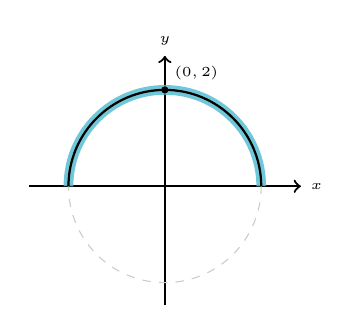
\begin{tikzpicture}[scale=0.72]
    \draw[->, thick] (-2.4,0) -- (2.4,0) node[right] {\tiny $x$};
    \draw[->, thick] (0,-2.1) -- (0,2.3) node[above] {\tiny $y$};
    \draw[gray!40, dashed] (0,0) circle (1.7);
    \draw[line width=3.5pt, chalkcyan!70, opacity=0.85] (1.7,0) arc (0:180:1.7);
    \draw[thick] (1.7,0) arc (0:180:1.7);
    \filldraw[black] (0,1.7) circle (1.5pt) node[above right] {\tiny $(0,2)$};
  \end{tikzpicture}
\end{minipage}%
\hfill
\begin{minipage}[c]{0.72\textwidth}
  \textbf{Top Hemisphere:} $y = \sqrt{4 - x^2} = (4 - x^2)^{1/2}$\\[1pt]
  $\text{inner: } 4 - x^2 \implies \text{inner}' = -2x, \quad \text{outer: } u^{1/2} \implies \text{outer}' = \tfrac{1}{2}u^{-1/2}$\\[1pt]
  \[
    \frac{dy}{dx} = \frac{1}{2}(4 - x^2)^{-1/2} \cdot (-2x) = \frac{-x}{\sqrt{4 - x^2}} = -\frac{x}{y} \quad \text{\footnotesize (since $y = \sqrt{4-x^2}$)}
  \]
\end{minipage}

\vspace{0.04in}
\textbf{Do the same for the point $(0,-2)$ (and $x = -1$):}

\begin{minipage}[c]{0.26\textwidth}
  \centering
  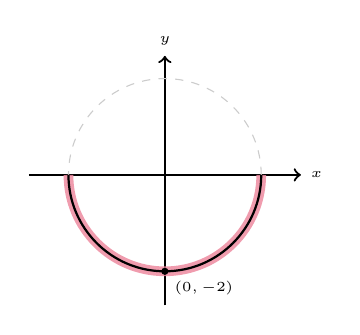
\begin{tikzpicture}[scale=0.72]
    \draw[->, thick] (-2.4,0) -- (2.4,0) node[right] {\tiny $x$};
    \draw[->, thick] (0,-2.3) -- (0,2.1) node[above] {\tiny $y$};
    \draw[gray!40, dashed] (0,0) circle (1.7);
    \draw[line width=3.5pt, chalkpink!70, opacity=0.85] (1.7,0) arc (0:-180:1.7);
    \draw[thick] (1.7,0) arc (0:-180:1.7);
    \filldraw[black] (0,-1.7) circle (1.5pt) node[below right] {\tiny $(0,-2)$};
  \end{tikzpicture}
\end{minipage}%
\hfill
\begin{minipage}[c]{0.72\textwidth}
  \textbf{Bottom Hemisphere:} $y = -\sqrt{4 - x^2} = -(4 - x^2)^{1/2}$\\[1pt]
  \[
    \frac{dy}{dx} = -\left( \frac{-x}{\sqrt{4 - x^2}} \right) = \frac{x}{\sqrt{4 - x^2}} = \frac{-x}{-\sqrt{4 - x^2}} = -\frac{x}{y} \quad \text{\footnotesize (since $y = -\sqrt{4-x^2}$)}
  \]
\end{minipage}

\vspace{0.04in}
\textbf{Notice that in both the above cases, across the entire circle, we can write:}
\[
  \frac{dy}{dx} = -\frac{x}{y}
\]

\vfill
\noindent \textbf{Math 105L} \hfill \textbf{Page 1 of 5}

\newpage

% ==============================================================================
% PAGE 2 (Page 2 of 5)
% ==============================================================================
\noindent \textbf{\large Math 105L} \hfill \textbf{\large Lecture 9-2}\\[2pt]
{\textbf{\Large Implicit Differentiation}}\\[-4pt]
\rule{\textwidth}{1.2pt}

\vspace{0.03in}

\textbf{\large The Implicit Differentiation Technique}

Even though $x^2 + y^2 = 4$ does not define $y$ as a function of $x$, it is still close to a function that the derivative makes sense, and the usual rules apply. Let's pretend $y$ is a function of $x$, differentiate both sides, and solve for $\frac{dy}{dx}$:

\begin{itemize}[leftmargin=1.2em, topsep=1pt, itemsep=2pt]
  \item \textbf{Write $y = y(x)$:} \quad $x^2 + \big(y(x)\big)^2 = 4$
  \item \textbf{Differentiate both sides with respect to $x$:} \quad $\frac{d}{dx}[x^2] + \frac{d}{dx}\left[\big(y(x)\big)^2\right] = \frac{d}{dx}[4]$
  \item \textbf{Chain Rule on the $y$-term:} \quad $\frac{d}{dx}\left[\big(y(x)\big)^2\right] = 2y(x) \cdot y'(x)$ \quad ($\text{inner: } y(x), \text{ outer: } u^2 \implies 2u \cdot u'$)
  \item \textbf{Solve for $y'(x)$:}
  \[
    2x + 2y(x) \cdot y'(x) = 0 \implies 2y(x) y'(x) = -2x \implies y'(x) = \frac{-2x}{2y(x)} = -\frac{x}{y}
  \]
\end{itemize}
\textit{Takeaway: Two lines of algebra, no square roots, and it works uniformly across the whole curve!}

\vspace{0.04in}
\textbf{\large Geometric Significance \& Why $\frac{dy}{dx}$ Depends on Both $x$ and $y$}
\begin{itemize}[leftmargin=1.2em, topsep=0pt, itemsep=1pt]
  \item Because the circle fails the vertical line test, a single $x$-value has multiple points on the curve:
  \begin{itemize}[leftmargin=1.2em, label=--, topsep=0pt, itemsep=1pt]
    \item At $(1, \sqrt{3})$ (top): $m = -\frac{1}{\sqrt{3}}$ (negative slope, tangent tilts downhill).
    \item At $(1, -\sqrt{3})$ (bottom): $m = -\frac{1}{-\sqrt{3}} = \frac{1}{\sqrt{3}}$ (positive slope, tangent tilts uphill).
  \end{itemize}
  \item \textbf{We also need the $y$-value} to determine which point on the curve we are evaluating!
\end{itemize}

\vspace{0.04in}
\textbf{\large Singularities: Vertical Tangent Lines}
\begin{itemize}[leftmargin=1.2em, topsep=0pt, itemsep=1pt]
  \item \textbf{Are there any points where $\frac{dy}{dx}$ is not defined? What happens to the tangent line at these points?}
  \begin{itemize}[leftmargin=1.2em, label=$\bullet$, topsep=0pt, itemsep=1pt]
    \item The derivative $\frac{dy}{dx} = -\frac{x}{y}$ is \textbf{undefined} when the denominator is zero: $y = 0$.
    \item Setting $y = 0$ in $x^2 + y^2 = 4 \implies x^2 + 0^2 = 4 \implies x = \pm 2$. Points: $(2,0)$ and $(-2,0)$.
    \item \textbf{Geometric Meaning:} At $(2,0)$ and $(-2,0)$, the tangent lines are \textbf{vertical lines} ($x = 2$ and $x = -2$).
  \end{itemize}
\end{itemize}

\vspace{0.04in}
\textbf{\large Revisit: $xy + y = e^x$ via Implicit Differentiation}
\begin{itemize}[leftmargin=1.2em, topsep=0pt, itemsep=1pt]
  \item \textbf{Question:} Let's revisit $xy + y = e^x$. What is $\frac{dy}{dx}$? Check that it's the same as what you got previously!
  \begin{itemize}[leftmargin=1.2em, label=$\bullet$, topsep=0pt, itemsep=1pt]
    \item \textbf{Write:} $x \cdot y(x) + y(x) = e^x$.
    \item \textbf{Differentiate via Product Rule on $x \cdot y(x)$:} $\frac{d}{dx}[x y(x)] = 1 \cdot y(x) + x y'(x)$.
    \[
      (y + x y') + y' = e^x \implies x y' + y' = e^x - y \implies y'(x+1) = e^x - y \implies y' = \frac{e^x - y}{x+1}
    \]
    \item \textbf{Check against explicit form:} Substitute $y = \frac{e^x}{x+1}$ into numerator:
    \[
      y' = \frac{e^x - \frac{e^x}{x+1}}{x+1} = \frac{\frac{e^x(x+1) - e^x}{x+1}}{x+1} = \frac{xe^x + e^x - e^x}{(x+1)^2} = \frac{xe^x}{(x+1)^2} \quad \checkmark
    \]
  \end{itemize}
\end{itemize}

\vspace{0.04in}
\begin{tcolorbox}[colback=boxbg, colframe=boxframe, boxrule=0.7pt, arc=2.5pt, left=6pt, right=6pt, top=4pt, bottom=4pt]
  \textbf{\large Implicit Differentiation (Summary Statement)}\\[2pt]
  What we carried out in these cases is a process of \textbf{implicit differentiation}:
  \begin{enumerate}[leftmargin=1.2em, topsep=1pt, itemsep=1pt]
    \item We implicitly assume that $y$ is a function of $x$ ($y = y(x)$), making expressions like $y^2, y^3, e^y, \dots$ compound functions: $y^2 = [y(x)]^2, \quad e^y = e^{y(x)}, \dots$
    \item We then use the \textbf{Chain Rule} to differentiate them: $\frac{d}{dx}[y^n] = n y^{n-1} \cdot y', \quad \frac{d}{dx}[e^y] = e^y \cdot y'$.
    \item We algebraically isolate all terms with $y'$ and solve for $\frac{dy}{dx}$.
  \end{enumerate}
\end{tcolorbox}

\vfill
\noindent \textbf{Math 105L} \hfill \textbf{Page 2 of 5}

\end{document}
